`% !TeX root = ../defense.tex

\section{Motivation}
\frame{\sectionpage}

\begin{frame}{Relative Turn Length}{Timing Diagram}
\begin{center}
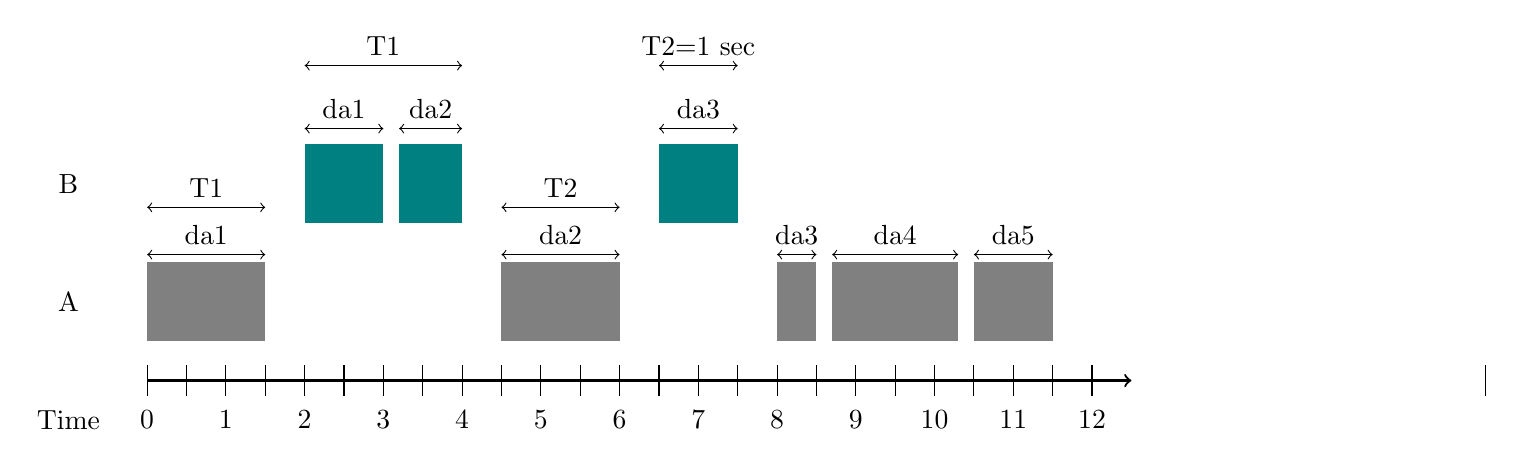
\begin{tikzpicture}
 %   \begin{axis}[
 %       tumaxisstyle,
 %       x post scale=1.75,
     %   ymin=0,ymax=3,
 %        xmin=0,xmax=24,
 %        xlabel={Time}]
     %   ylabel={Turns}]
 %    \end{axis}
    \draw [->, thick, black] (0,0) -- (12.5,0);
    \draw (0,-.2) -- (0, .2);
    \draw (0.5,-.2) -- (0.5, .2);
    \draw (1,-.2) -- (1, .2);
    \draw (1.5,-.2) -- (1.5, .2);
    \draw (2,-.2) -- (2, .2);
    \draw (2.5,-.2) -- (2.5, .2);
    \draw (3,-.2) -- (3, .2);
    \draw (3.5,-.2) -- (3.5, .2);
    \draw (4,-.2) -- (4, .2);
    \draw (4.5,-.2) -- (4.5, .2);
    \draw (5,-.2) -- (5, .2);
    \draw (5.5,-.2) -- (5.5, .2);
    \draw (6,-.2) -- (6, .2);
    \draw (6.5,-.2) -- (6.5, .2);
    \draw (7,-.2) -- (7, .2);
    \draw (7.5,-.2) -- (7.5, .2);
    \draw (8,-.2) -- (8, .2);
    \draw (8.5,-.2) -- (8.5, .2);
    \draw (9,-.2) -- (9, .2);
    \draw (9.5,-.2) -- (9.5, .2);
    \draw (10,-.2) -- (10, .2);
    \draw (10.5,-.2) -- (10.5, .2);
    \draw (11,-.2) -- (11, .2);
    \draw (11.5,-.2) -- (11.5, .2);
    \draw (12,-.2) -- (12, .2);
    
    \draw (17,-.2) -- (17, .2);

    \node at (-1,-0.5) {Time};
    \node at (0,-0.5) {0};
    \node at (1,-0.5) {1};
    \node at (2,-0.5) {2};
    \node at (3,-0.5) {3};
    \node at (4,-0.5) {4};
    \node at (5,-0.5) {5};
    \node at (6,-0.5) {6};
    \node at (7,-0.5) {7};
    \node at (8,-0.5) {8};
    \node at (9,-0.5) {9};
    \node at (10,-0.5) {10};
    \node at (11,-0.5) {11};
    \node at (12,-0.5) {12};
    
    \node at (-1,1) {A};
    \node at (-1,2.5) {B};
    
    %A turn 1 , 0 - 1.5 sec with one da
    \uncover<1->{%
      \path [fill=gray] (0,0.5) rectangle (1.5,1.5);
    }
    
    \uncover<2->{%
        \draw [<->] (0,2.2) -- node[above] {T1} (1.5,2.2);
        \draw [<->] (0,1.6) -- node[above] {da1} (1.5,1.6);
    }
    
    %B turn 1, da1  2 - 3
    \uncover<3->{%
       \path [fill=teal] (2,2) rectangle (3,3);
       \draw [<->] (2,3.2) -- node[above] {da1} (3,3.2);    
    }
     
        
    %B turn 1, da2 3.2 - 4 
    \uncover<4->{%
        \path [fill=teal] (3.2,2) rectangle (4,3);
        \draw [<->] (3.2,3.2) -- node[above] {da2} (4,3.2);
    }

    \uncover<5->{%
            \draw [<->] (2,4) -- node[above] {T1} (4,4);
    }

    
    % A turn 2 4.5 - 6
    \uncover<6->{%
       \path [fill=gray] (4.5,0.5) rectangle (6,1.5);
    }
    
    % A turn 2 4.5 - 6 , header
    \uncover<7->{%
        \draw [<->] (4.5,2.2) -- node[above] {T2} (6,2.2);
        \draw [<->] (4.5,1.6) -- node[above] {da2} (6,1.6);
    }
    
    
    %B turn 2 6.5 - 7.5
    \uncover<8->{%
       \path [fill=teal] (6.5,2) rectangle (7.5,3);
    }
    
    %B turn 2 6.5 - 7.5 header
    \uncover<9->{%
        \draw [<->] (6.5,3.2) -- node[above] {da3} (7.5,3.2);
        \draw [<->] (6.5,4) -- node[above] {T2=1 sec} (7.5,4);
    }
    
    %A turn 3, da3
    \uncover<10->{%
       \path [fill=gray] (8,0.5) rectangle (8.5,1.5);
       \draw [<->] (8,1.6) -- node[above] {da3} (8.5,1.6);
    }
    
    %A turn 3, da4
    \uncover<11->{%
       \path [fill=gray] (8.7,0.5) rectangle (10.3,1.5);
       \draw [<->] (8.7,1.6) -- node[above] {da4} (10.3,1.6);
    }
    
    \uncover<12->{%
       \path [fill=gray] (10.5,0.5) rectangle (11.5,1.5);
       \draw [<->] (10.5,1.6) -- node[above] {da5} (11.5,1.6);
    }
    

    % original wind timeseries
%    \addplot[name path=ts-wind,draw=none,const plot]
%        coordinates { \windts };

%    \addplot[name path=ts-wind-half,draw=none,const plot,
%             y filter/.code={\pgfmathparse{\pgfmathresult/2}\pgfmathresult}]
%        coordinates {\windts };

    % finally: demand plot
%    \addplot[name path=ts-demand,draw=demand,const plot] coordinates { \demandts };
%    % slide-show

%    \only<2-5>{%
%        \addplot[fill=wind] fill between[of=axis and ts-wind-half];
%    }
%    \only<2-4>{%
%        \node[jdblack] at (12,1) {Wind turbine};
%    }
%
%    \only<3-5>{%
%        \addplot[fill=gas] fill between[of=ts-wind-half and ts-demand];
%    }
%    \only<3-4>{%
%        \node[jdwhite!95!gas] at (12,4.5) {Gas plant};
%    }

%    \only<6->{%
%        \addplot[fill=wind] fill between[of=axis and ts-wind];
%        \addplot [fill=gas] fill between[of=ts-wind and ts-demand,split,
%                        every segment no 2/.style={fill=none},
%                        every segment no 5/.style={fill=none}];
%    }

%    \only<7|handout:0>{%
%        \draw[jdblack!75!wind,thick,darrows] (4.5, 0) -- node[right] {$\kappa_\text{w} = 8$} (4.5, 8);
%        \draw[jdwhite!95!gas,thick,darrows] (20.5, 0) -- node[right] {$\kappa_\text{g} = 9$} (20.5, 9);
%    }

 %   \only<9->{%
 %       \fill[storage!50] (4, 0) -- (4, 4)
 %   }

%    \only<10->{%
%        \draw[jdblack!75!wind,thick,darrows] (4.5, 0) -- node[right] {$\kappa_\text{w} = 8$} (4.5, 8);
%        \draw[jdwhite!95!gas,thick,darrows] (20.5, 0) -- node[right] {$\kappa_\text{g} = 5$} (20.5, 5);
%    }

%    \only<11>{%
%        \node[jdblack!85!storage] at (5.5, -1) {$\kappa^\text{c}_\text{s} = 7$};
%        \draw[jdblack!85!storage,thick,darrows] (20.5, 5) -- node[right,near end,text=jdblack,xshift=.5em]
%            {$\kappa^\text{p}_\text{s} = 4$} (20.5, 9);
%    }

%    \addplot[draw=demand,thick,const plot] coordinates { \demandts };
%    \draw[black] (0,0) -- (24,0);
%  \end{axis}
\end{tikzpicture}
\end{center}
\end{frame}





\begin{frame}{Current Issues}
    \begin{enumerate}[<+->]\itemsep9pt
      \item For a natural conversation between human and machine, we want to conform
            to human to human turn taking system (Sacks et al, 1978)
      \item In Human-Human conversations conversant predict (Sacks et al, 1978) or
            signal (Duncan 1972) each other on coming turn transition
      \item {
        Timeouts leads to poor user interaction(Arsikere et al, 2015)
        \begin{itemize}
            \item Not effective in noisy environment
            \item too little - machine barge in during intra turn pause.
            \item too much - user waiting for the machine.
        \end{itemize}
      }
      \item {
        Turn transition prediction based on local features improve turn taking but still
        do not match human performance.
        \begin{itemize}
            \item Syntactic (Sacks et al 1978,De Ruiter et al. 2006)
            \item Prosodic (Ford 1996,Stolcke 2002,Ferrer 2003)
            \item Pragmatic (Ford 2001)
        \end{itemize}
      }
    \end{enumerate}
\end{frame}

\begin{frame} {Goal of Work}
        Conversant's past behavior can help predict turn transitions

        Past behavior represented by Summary features
\end{frame}
